%allgemeine Formatangaben
\documentclass[
 a4paper, 										% Papierformat
 12pt,												% Schriftgröße
 ngerman, 										% für Umlaute, Silbentrennung etc.
 titlepage,										% es wird eine Titelseite verwendet
 oneside, 										% einseitiges Dokument
 captions=nooneline,					% einzeilige Gleitobjekttitel ohne Sonderbehandlung wie mehrzeilige Gleitobjekttitel behandeln
 numbers=noenddot,						% Überschriften-??Nummerierung ohne Punkt am Ende
 parskip=half,									% zwischen Absätzen wird eine halbe Zeile eingefügt
 ]{scrartcl}


% Anpassung an Landessprache
\usepackage[ngerman]{babel}	

\usepackage[T1]{fontenc}	
\usepackage[utf8]{inputenc}	
\usepackage{textcomp} 																% Euro-Zeichen und andere
\usepackage[babel,german=quotes]{csquotes}						% Anführungszeichen
\RequirePackage[ngerman=ngerman-x-latest]{hyphsubst} 	% erweiterte Silbentrennung

\usepackage{tocloft} %Wird benötigt damit das veränderte Counterverhalten nicht mit Text überlappt!
\usepackage{etoolbox} %Url Umbruch im Bibtex!

% Befehle aus AMSTeX für mathematische Symbole z.B. \boldsymbol \mathbb
\usepackage{amsmath,amsfonts}

% Zeilenabstände und Seitenränder 
\usepackage{setspace}
\usepackage{geometry}

% Einbinden von JPG-Grafiken
\usepackage{graphicx}

% zum Umfließen von Bildern
% Verwendung unter http://de.wikibooks.org/wiki/LaTeX-Kompendium:_Baukastensystem#textumflossene_Bilder
\usepackage{floatflt}

% Verwendung von vordefinierten Farbnamen zur Colorierung
% Palette und Verwendung unter http://kitt.cl.uzh.ch/kitt/CLinZ.CH/src/Kurse/archiv/LaTeX-Kurs-Farben.pdf
\usepackage[usenames,dvipsnames]{color} 

% Tabellen
\usepackage{array}
\usepackage{longtable}

% einfache Grafiken im Code
% Einführung unter http://www.math.uni-rostock.de/~dittmer/bsp/pstricks-bsp.pdf
%\usepackage{pstricks}


% Quellcodeansichten
%\usepackage{verbatim}
%\usepackage{moreverb} 											% für erweiterte Optionen der verbatim Umgebung
% Befehle und Beispiele unter http://www.ctex.org/documents/packages/verbatim/moreverb.pdf
%\usepackage{listings} 											% für angepasste Quellcodeansichten siehe
% Kurzeinführung unter http://blog.robert-kummer.de/2006/04/latex-quellcode-listing.html



% verlinktes und Farblich angepasstes Inhaltsverzeichnis
\usepackage[pdftex,
colorlinks=true,
linkcolor=InterneLinkfarbe,
urlcolor=ExterneLinkfarbe]{hyperref}
\usepackage[all]{hypcap}

% URL verlinken, lange URLs umbrechen
\usepackage{url}

% sorgt dafür, dass Leerzeichen hinter parameterlosen Makros nicht als Makroendezeichen interpretiert werden
\usepackage{xspace}

% Beschriftungen für Abbildungen und Tabellen
%\usepackage{caption}

%\usepackage{chngcntr}
%Ändert counterverhalten von figure, table usw..

% Entwicklerwarnmeldungen entfernen
%\usepackage{scrhack}
% Glossar und Abbildungsverzeichnis
%\usepackage[
%nonumberlist, %keine Seitenzahlen anzeigen
%acronym,      %ein Abkürzungsverzeichnis erstellen
%toc          %Einträge im Inhaltsverzeichnis
%]      %im Inhaltsverzeichnis auf section-Ebene erscheinen
%{glossaries}
\usepackage{makeidx}
\makeindex

\usepackage{amsmath, amssymb}

\usepackage[printonlyused]{acronym}					% einbinden der verwendeten Latex-Pakete
\newcommand{\qq}[1]{\glqq{#1\grqq{}}} %Gänsefüßchen
\newcommand{\idx}[1]{#1\index{#1} } % Index drucken und schreiben

\onehalfspacing 							% 1,5facher Zeilenabstand

\definecolor{InterneLinkfarbe}{rgb}{0.1,0.1,0.3} 	% Farbliche Absetzung von externen Links
\definecolor{ExterneLinkfarbe}{rgb}{0.1,0.1,0.7}	% Farbliche Absetzung von internen Links

% Einstellungen für Fußnoten:
\captionsetup{font=footnotesize,labelfont=sc,singlelinecheck=true,margin={5mm,5mm}}

% Quellenangaben Stil
\bibliographystyle{alphadin}

%Ausschluss von Schusterjungen
\clubpenalty = 10000
%Ausschluss von Hurenkindern
\widowpenalty = 10000


% Beispiel für eine Listings-Codeumbebungen
% Bei mehreren Definitionen empfielt sich das auslagern in eine externe Datei
\lstloadlanguages{C++}
\lstset{
	frame=tb,
	framesep=5pt,
	basicstyle=\footnotesize\ttfamily,
	showstringspaces=false,
	keywordstyle=\ttfamily\bfseries %\color{CadetBlue},
	identifierstyle=\ttfamily,
	stringstyle=\ttfamily %\color{OliveGreen},
	%commentstyle=\color{GrayBlue},
%	rulecolor=\color{Gray},
	xleftmargin=5pt,
	xrightmargin=5pt,
	aboveskip=\bigskipamount,
	belowskip=\bigskipamount
} 

%Den Punkt am Ende jeder Beschreibung deaktivieren
\renewcommand*{\glspostdescription}{}

\setlength{\cftfignumwidth}{3em} %Befehl von tocloft
\setlength{\cfttabnumwidth}{3em}
%Counter verhalten verändern
\counterwithin{figure}{section}
\counterwithin{table}{section}

%Glossar-Befehle anschalten
\makeindex
\makeglossaries
\glsenablehyper

\apptocmd{\UrlBreaks}{\do\f\do\m}{}{}
						

\begin{document}


\title{Entwicklung eines IR-Empfänger und -Sender mit dem ESP8266}
\subtitle{Dokumentation: Microcontroller-Anwendungs-Projekt}
\author{} %TODO Später hinzufügen
\date{\today}

\maketitle

\tableofcontents										% Inhaltsverzeichnis
\pagebreak
%\listoffigures											% Abbildungsverzeichnis
%\pagebreak
%\listoftables											% Tabellenverzeichnis
%\pagebreak

\section{Einleitung}
\subsection{Ausgangspunkt}
Als Ausgangspunkt des Projektes ist die Absicht eine Infrarot-Fernbedingung mit Hilfe eines Mikrocontrollers zu realisieren.
Dieser soll über eine Website im heimischen Netzwerk angesprochen und entsprechend gesteuert werden können.

Zur Umsetzung dieses Vorhabens bietet sich der Mikrocontroller ESP8266 an.
Dieser Mikrocontroller ist preiswert und besitzt ein integriertes WLAN-Modul.

\subsection{Ziele}
Ziel des Projektes ist es, eine Schaltung einschließlich dazugehöriger Mikrocontroller-Software zu entwickeln, die folgende Funktionen bietet:

\begin{itemize}
	\item Mikrocontroller muss Netzwerkfunktionalität als Server bieten
	\item Kommunikation mit Server über drahtloses Netzwerk
	\item AccessPoint zur Konfiguration des ESP8266
	\item Einwahl in vorhandenes drahtloses Netzwerk und Speichern der Einwahldaten
	\item Steuerung des ESP8266 über Website
	\item Erfassen, Speichern und Ausgabe von Infrarot-Signalen (38kHz)
\end{itemize}

Alle diese Ziele sind mit Hilfe eines ESP8266 und weiterer Komponenten realisierbar.

\section{Grundlagen}
\subsection{Der ESP8266}
Der ESP8266 ist ein kostengünstiger programmierbarer WLAN-System-on-a-Chip mit einer UART-und SPI-Schnittstelle.
Ursprünglich wurde dieser SoC von Espressif entwickelt und verkauft, inzwischen bieten aber verschiedene andere Hersteller ebenfalls Varianten vom ESP8266 an.
Diese SoC sind ab einem Preis von ca. 4€ verfügbar.

Nachfolgend ist die Spezifikation eines ESP8266 laut Hersteller gelistet:

\begin{itemize}
	\item 802.11 b/g/n
    \item Wi-Fi Direct (P2P), soft-AP
    \item Integrated TCP/IP protocol stack
    \item Integrated TR switch, balun, LNA, power amplifier and matching network
    \item Integrated PLLs, regulators, DCXO and power management units
    \item +19.5dBm output power in 802.11b mode
    \item Power down leakage current of <10uA
    \item Integrated low power 32-bit CPU could be used as application processor
    \item SDIO 1.1/2.0, SPI, UART
    \item STBC, 1×1 MIMO, 2×1 MIMO
    \item A-MPDU \& A-MSDU aggregation \& 0.4ms guard interval
    \item Wake up and transmit packets in < 2ms
    \item Standby power consumption of < 1.0mW (DTIM3)
    \item VCC: 3,3V (Nicht 5V tolerant)
\end{itemize}
(Quelle: \url{http://www.mikrocontroller.net/articles/ESP8266} ; Stand: 18.01.2016)
Verfügbare Flash-Größe, Arbeitsspeicher und CPU-Frequenz sind Modell abhängig.

In der \autoref{fig:ESP8266} ist ein ESP8266 mit dem dazugehörigen Pinlayout dargestellt.

\begin{figure}
	\centering
	\begin{minipage}{0.45\textwidth}
			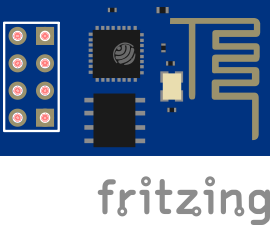
\includegraphics[scale=1.5]{Abbildungen/ESP8266A}
	\end{minipage}
	\hfill
	\begin{minipage}{0.45\textwidth} 
			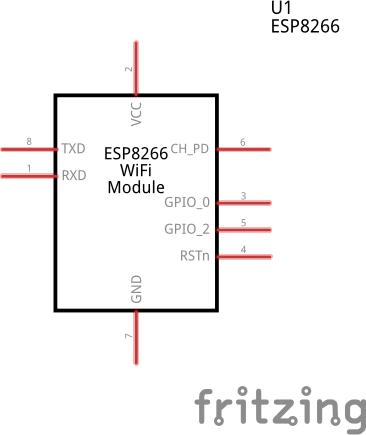
\includegraphics[scale=1.5]{Abbildungen/ESP8266}
	\end{minipage}
	\caption{ESP8266 Platine und Schaltung}
	\label{fig:ESP8266}
\end{figure}

\subsection{Programmierung}
Die Programmierung des Mikrocontrollers erfolgt mit der Arduino IDE.
Zu finden ist diese IDE unter \url{https://www.arduino.cc/} (Stand: 18.01.2016).

Weiterhin wird der ESP8266 über die TXD- und RXD-Leitungen mit Hilfe des UART-Protokolls programmiert.
Damit der Controller in den Programmiermodus wechselt, muss beim Start der GPIO\_0 auf Masse liegen.
Anschließend kann die durch Cross-Compiling erzeugte Binary der Arduino Entwicklungsumgebung innerhalb der IDE an den ESP8266 übertragen werden.
Für die Programmierung bieten sich beispielsweise sogenannte USB-to-UART-Programmierkabel an (beispielsweise der PL2303).
Wichtig: VCC solcher Kabeln liefern üblicherweise 5V! Der Mikrocontroller ist nicht 5V tolerant.
Für den normalen Betrieb des ESP8266 muss GPI0\_0 auf High liegen.

\subsection{Funktionsweise Infrarot}
Damit eine WLAN-gesteuerte Infrarotfernbedingung realisiert werden kann, müssen zunächst die Grundlagen einer solchen Fernbedingung kurz erklärt werden.

Eine Infrarot-Fernbedienung sendet über eine Infrarotleuchtdiode ein Signal im Infrarotbereich.
Dieses Signal wird mit einer bestimmten Trägerfrequenz gesendet.
Viele Fernbedingungen arbeiten beispielsweise mit einer Trägerfrequenz von 38kHz.
Es existieren aber Fernbedingungen, welche andere Frequenzen nutzen.
In diesem Projekt wird eine Fernbedingung mit 38kHz realisiert.
Es ist wichtig sich auf eine Frequenz festzulegen, da die Frequenz Einfluss auf Bauteile und Programmierung hat.

Über eine \textbf{P}uls-\textbf{W}eiten-\textbf{M}odulation (PWM) auf der Trägerfrequenz wird das codierte Signal übertragen.
Jede Taste auf einer Fernbedingung besitzt eine eigene Codierung.
Weiterhin existieren verschiedene Protokolle zur Codierung von Signalen.
Die Protokolle werden in diesem Projekt vernachlässigt, da die Codierung im Wesentlichen nur kopiert und gespeichert wird.

Damit das Infrarotsignal empfangen werden kann, wird ein entsprechender Empfänger benötigt.
Solche Empfänger sind als integrierte Schaltkreise verfügbar, welche alle benötigten Funktionen in einem Bauteil vereinen.
Ein Infrarotempfänger besteht aus einer Fotodiode, einem geregeltem Verstärker, welcher entsprechend der Frequenz arbeitet (zum Beispiel 38kHz) und einem Demodulator.
Der Demodulator sendet das digital codierte Signal an den Mikrocontroller.
Weiterhin besitzt der integrierte Schaltkreis einen Bandpassfilter um Störungen von anderen Frequenzen als der gewünschten Frequenz zu vermeiden.
Meist sind Fotodiode und Schaltkreis in einem Kunststoffgehäuse integriert.
Der TSOP4836 ist zum Beispiel solch ein Empfänger für die Trägerfrequenz von 38kHz.

%ESP8266 Modul hat 2 Digitale Ein/Ausgänge. GPO2 benutzen wir als Eingang.
%Warum wird GPO0 als low aktiv benutzt? GPO0 wird für das Aktivieren der Firmware Update verwendet. So das für normale Betrieb des ESP8266 Moduls nach dem Reset immer HIGH Pegel anliegen soll.

\section{Realisierung}
Nachdem die Grundlagen für das Projekt betrachtet wurden, soll nun die konkrete Realisierung des Projektes verdeutlicht werden.

\subsection{Aufbau}
Die \autoref{fig:Schalplan} zeigt den Schaltplan für die Realisierung einer Infrarot-Fernbedingung inklusive Empfänger.

\begin{figure}
	\centering
	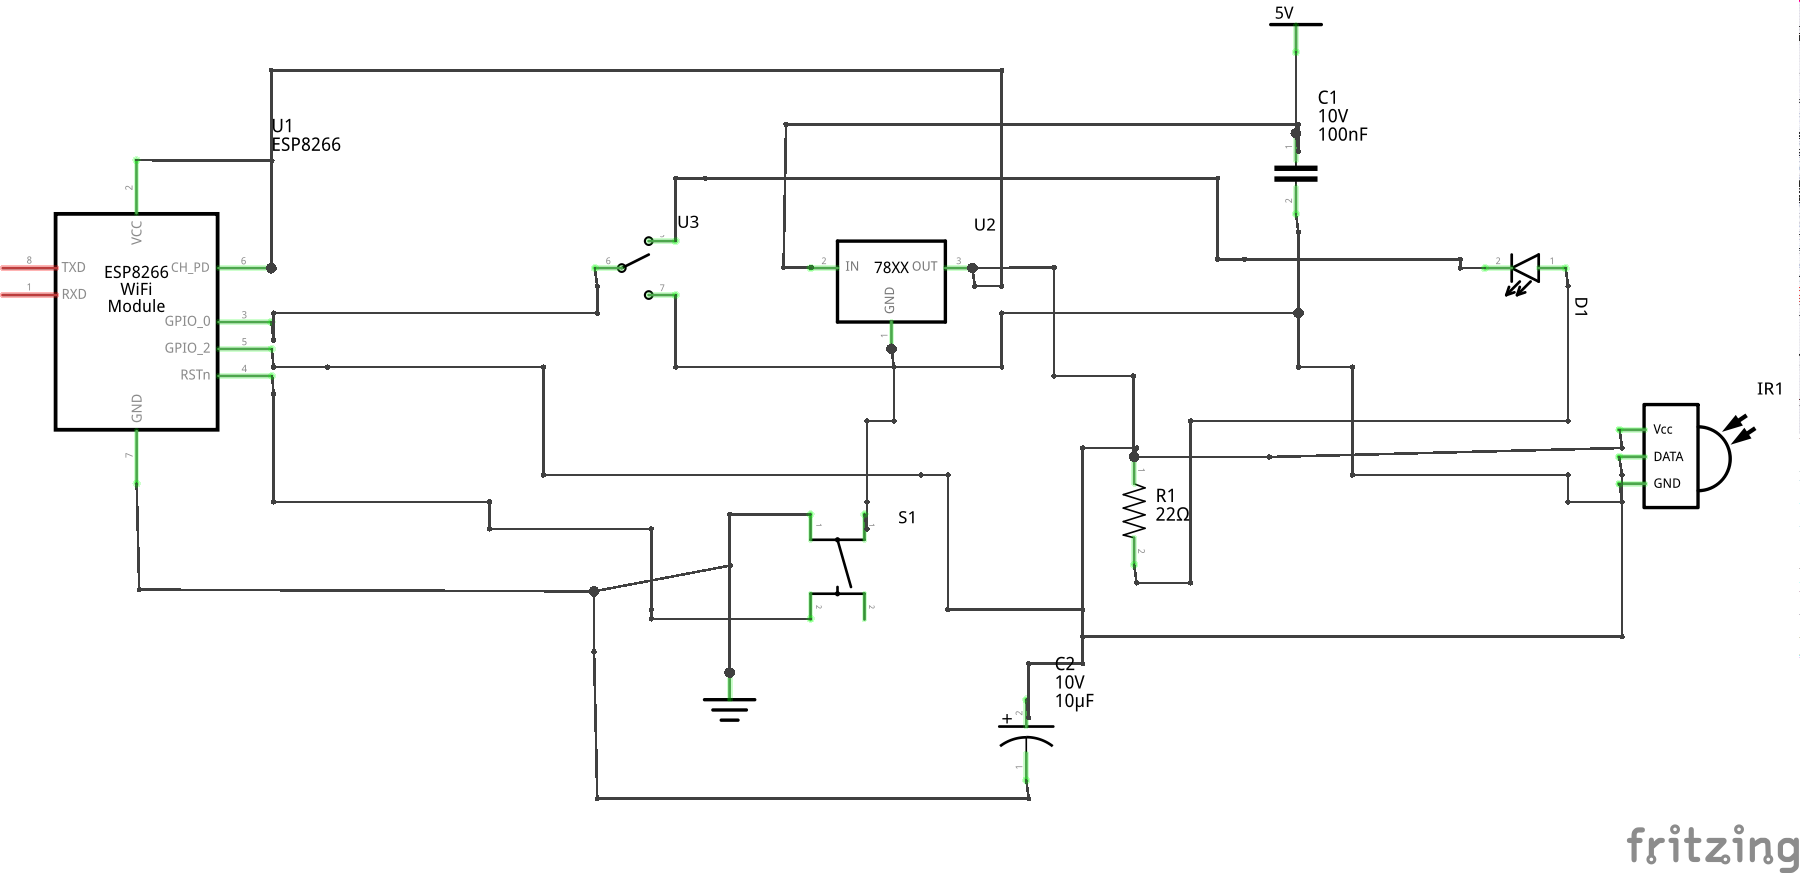
\includegraphics[scale=1]{Abbildungen/ESP8266_Schaltplan}
	\caption{Schaltplan}
	\label{fig:Schalplan}
\end{figure}

Für die Programmierung des Mikrocontrollers wird ein USB-to-UART-Programmierer (PL2303) verwendet.
Dieser liefert an VCC 5V.
Der ESP8266 selbst benötigt 3,3V und ist nicht 5V tolerant, sodass ein fester Spannungsregler verwendet wird um 3,3V für den Mikrocontroller zur Verfügung zu stellen.
Als Spannungsregler bietet sich zum Beispiel der LM1117-3V3 (verwendet) oder ein L7805 an.
%http://www.ti.com/lit/ds/symlink/lm1117.pdf
Der Spannungsregler ist im Schaltplan als 78XX dargestellt.
Zur Spannungsstabilisierung besitzt der Spannungsregler zwischen Out und GND einen 10$\mu$F-Kondensator.
Nun wird für den ESP8266 die benötigte Spannung von 3,3V bereitgestellt.
%TODO Schaltplan!!
Die Pins VCC und CHPD (Chip Power Down) werden mit der Spannungsquelle 3,3V verbunden und GND entsprechend auf Masse gelegt.
Der RST-Pin (Reset) wird mit einem Taster verbunden, welcher bei betätigen diesen Pin auf Masse zieht (interner Pull Up) und somit den Mikrocontroller zurücksetzt.
An dem GPIO\_0 ist ein DIP Schalter angeschlossen.
Dieser dient dazu zwischen dem Programmiermodus und dem normalen Modus zu Wechseln.
DerPin wird als Low aktiv benutzt, sodass für den normalen Betrieb und nach einem Reset immer High Pegel anliegen muss.
Für das Programieren wird dieseer PIN auf Masse gezogen in dem der Schalter entsprechend gesetzt wird.
Andernfalls ist der PIN mit einer Infrarotdiode (1,5V, 80mA) inklusive Vorwiederstand(22 Ohm) verbunden.
Diode und Wiederstand mit der 3,3V Spannungsquelle verbunden.

Diese Diode dient später dazu die Infrarotsignale zu senden, in dem der GPIO\_0 als Ausgang verwendet wird.

Der GPIO\_0 2 wird mit dem Infrarotempfänger verbunden, daher fungiert dieser PIN als Eingang zur Erfassung der Infrarot-Signale.
Der Infrarotempfänger wird entsprechend mit der 3,3V Spannungsquelle und der Masse verbunden.

Aufgrund das Senden und Empfangen nicht gleichzeitg möglich sind, bedarf es keiner Abschirmung zwischen Sender und Empfänger.

Die \autoref{fig:Steckplatine} zeigt den Aufbau auf einer Steckplatine

\begin{figure}
	\centering
	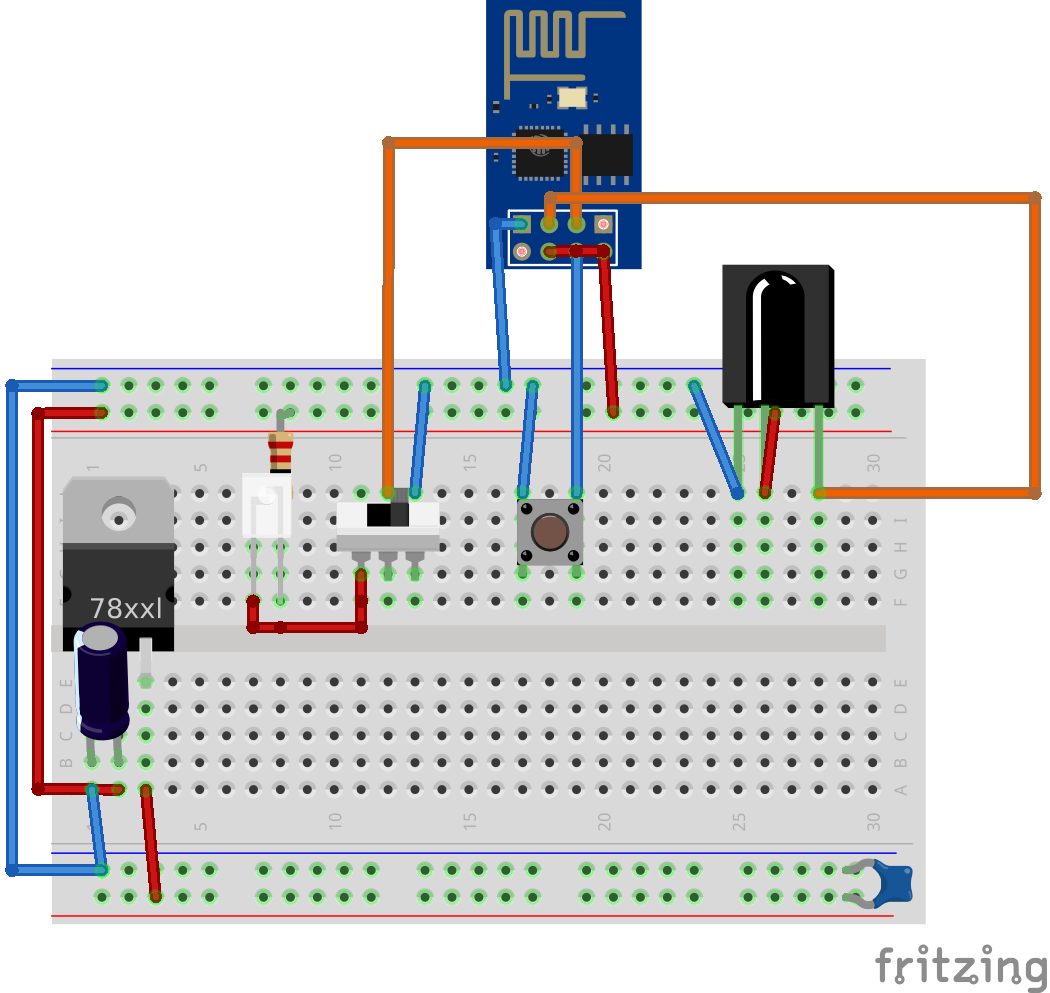
\includegraphics[scale=1]{Abbildungen/ESP8266_Steckplatine}
	\caption{Steckplatine}
	\label{fig:Steckplatine}
\end{figure}





\subsection{Implementierung}
%Programmablaufplan
Fortunately, there is a way around this ESP8266 constraint. The trick is to create the 38 kHz modulation by simply toggling a digital output; logic 1 and logic 0. The duration of these pulses determine the command sent to the remote receiver. But how do we generate 38 kHz pulses?

Simple…

Using the ESP8266 micro-second delay statement “os\_delay\_us(us)”, we can create a 38 kHz pulse train. Each pulse period is 1/38000 seconds (26.3 us) long. Rounding that off to 26 us, the modulation frequency is easily achieved with:

\subsection{Verwendung}
%Screenshots browser, verwendung beschreiben
\section{Zusammenfassung}
%todo footmarks für quellen und erklärungen von begriffen
\pagestyle{empty}										% Leere Seite 
\end{document}